\subsection{Caching and Memory-Mapped Devices}
\label{sec:memory_io}

The Intel architecture provides a few methods for specifying the cache behavior
for various ranges of the memory address space (\S~\ref{sec:address_spaces}).
This is used for memory mapped to devices, such as a graphics unit's
framebuffer. Caching framebuffer memory is indesirable, because the delay
between the time when a write is issued and the time when the corresponding
cache lines are evicted and written back to memory could lead to visual
artifacts on the user's display. This section covers the cacheability
mechanisms presented in the SDM, because understanding them is important for
analyzing SGX.


\subsubsection{Caching Behaviors}
\label{sec:cacheability_options}

% Memory-Mapped I/O: SDM vol1 S 16.3.1
% Methods of Caching Available: SDM S 11.3
% Ordering I/O: SDM vol1 S 16.6

\textit{Uncacheable} (UC) memory has the same semantics the I/O address space
(\S~\ref{sec:address_spaces}). UC memory is useful when a device's behavior is
dependent on the order of memory reads and writes, such as in the case of
memory-mapped command and data registers for a PCIe NIC
(\S~\ref{sec:motherboard}). The out of order execution engine
(\S~\ref{sec:out_of_order}) does not reorder UC memory accesses, and does not
issue speculative reads to UC memory.

\textit{Write Combining} (WC) memory addresses the specific needs of
framebuffers. WC memory is similar to UC memory, but the out of order engine
may reorder memory accesses, and may perform speculative reads. The processor
stores writes to WC memory in a write combining buffer, and attempts to group
multiple writes into a (more efficient) line write bus transaction.

\textit{Write Through} (WT) memory is cached, but write misses do not cause
cache fills. This is useful for preventing large memory-mapped device memories
that are rarely read, such as framebuffers, from taking up cache memory. WT
memory is covered by the cache coherence engine, may receive speculative reads,
and is subject to operation reordering.

DRAM is represented as \textit{Write Back} (WB) memory, which is optimized
under the assumption that all the devices that need to observe the memory
operations participate in the cache coherence protocol. WB memory is cached as
described in \S~\ref{sec:caching}, receives speculative reads, and operations
targeting it are subject to reordering.

\textit{Write Protected} (WP) memory is similar to WB memory, with the
exception that every write is propagated to the system bus. It is intended for
memory-mapped buffers, where the order of operations does not matter, but the
devices that need to observe the writes cannot participate in the cache
coherence protocol.


\subsubsection{Memory Caching Configuration}
\label{sec:cacheability_config}

% Cache Control Registers and Bits: SDM S 11.5.1
% Memory Type Range Registers (MTRRs): SDM S 11.11
% PCD and PWT Flags: SDM S 20.30.2

On recent Intel processors, the cache's behavior is mainly configured by the
\textit{Memory Type Range Registers} (MTRRs) and by
\textit{Page Attribute Table} (PAT) indices in the page tables
(\S~\ref{sec:paging}). The behavior is also impacted by the Cache Disable (CD)
and Not-Write through (NW) bits in Control Register 0
(CR0, \S~\ref{sec:address_spaces}), as well as by equivalent bits in page table
entries, namely Page-level Cache Disable (PCD) and Page-level Write-Through
(PWT).

The MTRRs were intended to be configurd by the computer's firmware during the
boot sequence. Fixed MTRRs cover pre-determined ranges of memory, such as the
areas that had special meaning in the computers using 16-bit Intel processors.
The ranges covered by \textit{variable MTRRs} can be configured by system
software. We describe the method used to specify these ranges, because the
principles behind it are also used by SGX.

% Variable Range MTRRs: SDM S 11.11.2.3
% Range Size and Alignment Requirement: SDM S 11.11.4

Each variable memory type range is specified using a \textit{range base} and a
\textit{range mask}. A memory address belongs to the range if computing a
bitwise AND between the address and the range mask results in the range base.
This verification has a low-cost hardware implementation, shown in
Figure~\ref{fig:mtrr_match}.

\begin{figure}[hbt]
  \center{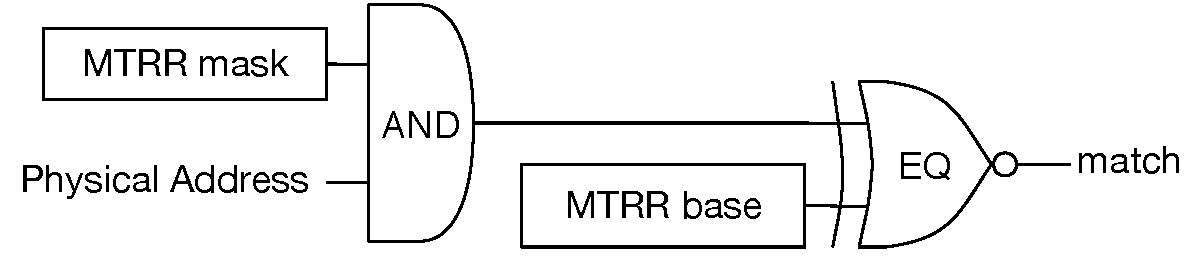
\includegraphics[width=85mm]{figures/mtrr_match.pdf}}
  \caption{
    The circuit for computing whether a physical address matches a memory type
    range.  Assuming a CPU with 48-bit physical addresses, the circuit uses 36
    AND gates and a binary tree of 35 XNOR (equality test) gates. The circuit
    outputs 1 if the address belongs to the range. The bottom 12 address
    bits are ignored, because memory type ranges must be aligned to 4KB page
    boundaries.
  }
  \label{fig:mtrr_match}
\end{figure}

Each variable memory type range must have a size that is an integral power of
two, and a starting address that is a multiple of its size, so it can be
described using the base / mask representation described above. A range's
starting address is its base, and the range's size is one plus its mask. No
memory type range can partially cover a 4KB page, which implies that the range
base must be a multiple of 4KB, and the bottom 12 bits of range mask must be
set. This simplifies the interactions between memory type ranges and address
translation, described in \S~\ref{sec:tlbs}.

The PAT is intended to allow the operating system or hypervisor to tweak the
caching behaviors specified in the MTRRs by the computer's firmware. The PAT
has 8 entries that specify caching behaviors, and is stored in its entirety in
a MSR. Each page table entry contains a 3-bit index that points to a PAT entry,
so the system software that controls the page tables can specify caching
behavior at a very fine granularity.

The SGX manual states that the EPC (the memory used to store enclave data) can
only be set up as UC or WB. While no further explanation is provided, we assume
that the UC option was provided in order to attempt to mitigate against some
cache-timing attacks.
